\documentclass[aspectratio=169,10pt]{beamer}

% ── Theme ────────────────────────────────────────────────────────────────────
\usetheme{Madrid}
\usecolortheme{whale}
\usefonttheme{professionalfonts}
\setbeamertemplate{navigation symbols}{}
\setbeamertemplate{footline}[frame number]
\setbeamertemplate{itemize items}[circle]

% ── Packages ─────────────────────────────────────────────────────────────────
\usepackage[utf8]{inputenc}
\usepackage[T1]{fontenc}
\usepackage{amsmath,amssymb}
\usepackage{booktabs}
\usepackage{tabularx}
\usepackage{graphicx}
\usepackage{subcaption}
\usepackage{xcolor}
\usepackage{tikz}
\usetikzlibrary{arrows.meta,positioning,calc,shapes.geometric,fit,backgrounds}
\usepackage{hyperref}
\usepackage{multirow}
\graphicspath{{../figures/}}

% ── Custom colours ───────────────────────────────────────────────────────────
\definecolor{autoBlue}{RGB}{30,80,140}
\definecolor{autoOrange}{RGB}{200,90,30}
\definecolor{autoGreen}{RGB}{40,140,80}
\definecolor{lightBlue}{RGB}{220,235,255}
\definecolor{lightOrange}{RGB}{255,235,215}
\definecolor{lightGreen}{RGB}{215,245,225}
\definecolor{codeGray}{RGB}{248,248,250}

\setbeamercolor{structure}{fg=autoBlue}
\setbeamercolor{palette primary}{bg=autoBlue,fg=white}
\setbeamercolor{palette secondary}{bg=autoBlue!80,fg=white}
\setbeamercolor{palette tertiary}{bg=autoBlue!60,fg=white}
\setbeamercolor{frametitle}{bg=autoBlue,fg=white}
\setbeamercolor{block title}{bg=autoBlue,fg=white}
\setbeamercolor{block body}{bg=lightBlue}
\setbeamercolor{block title alerted}{bg=autoOrange,fg=white}
\setbeamercolor{block body alerted}{bg=lightOrange}
\setbeamercolor{block title example}{bg=autoGreen,fg=white}
\setbeamercolor{block body example}{bg=lightGreen}

% ── Title ────────────────────────────────────────────────────────────────────
\title[AutoFOAM]{\textbf{AutoFOAM}: The Self-Refining Autonomous OpenFOAM Agent}
\subtitle{Bridging Natural Language and Computational Fluid Dynamics}
\author[Neelan \& Seshaditya]{Arun Govind Neelan$^{1}$ \and A Seshaditya$^{2,3}$}
\institute[SimuNetics]{
  $^{1}$SimuNetics, Kanyakumari, Tamil Nadu, India \\
  $^{2}$Onnes Cryogenics, Hyderabad, India \quad
  $^{3}$Quasi AI, Berlin, Germany
}
\date{}

% ─────────────────────────────────────────────────────────────────────────────
\begin{document}

% ── Title slide ──────────────────────────────────────────────────────────────
\begin{frame}
  \titlepage
  \begin{center}
    \small
    \texttt{arungovindneelan@gmail.com} \quad
    \texttt{adi@onnes.in / aditya@quasi.digital}
  \end{center}
\end{frame}

% ── Outline ──────────────────────────────────────────────────────────────────
\begin{frame}{Outline}
  \tableofcontents
\end{frame}

% =============================================================================
\section{Motivation}
% =============================================================================

\begin{frame}{The OpenFOAM Expertise Barrier}
  \begin{columns}
    \begin{column}{0.55\textwidth}
      \begin{block}{Why CFD is Hard to Access}
        \begin{itemize}
          \item OpenFOAM: unmatched flexibility for physics simulation
          \item Requires mastery of dozens of \textbf{C++ dictionaries}
          \item Syntax is \textbf{strict and deeply interconnected}
          \item Moving from physics idea $\to$ working simulation is \\ tedious and error-prone
        \end{itemize}
      \end{block}
      \vspace{4pt}
      \begin{alertblock}{Where Generic LLMs Fall Short}
        \begin{itemize}
          \item Invent non-existent OpenFOAM keywords
          \item Inconsistent boundary conditions across files
          \item Lack physical understanding of flow regimes
        \end{itemize}
      \end{alertblock}
    \end{column}
    \begin{column}{0.42\textwidth}
      \begin{exampleblock}{The Vision}
        \centering\vspace{6pt}
        \large
        \textit{``Simulate a turbulent flow over a NACA0012 airfoil at Re$= 10^6$''}\\[8pt]
        $\Downarrow$\\[6pt]
        \textbf{Full, convergent OpenFOAM case}\\
        \textit{generated autonomously}
        \vspace{6pt}
      \end{exampleblock}
      \vspace{4pt}
      \begin{block}{Related Work}
        \small
        FoamGPT, OpenFOAMGPT, Foam-Agent 2.0 — growing momentum for LLM-driven CFD
      \end{block}
    \end{column}
  \end{columns}
\end{frame}

% =============================================================================
\section{System Architecture}
% =============================================================================

\begin{frame}{AutoFOAM: The Eight-Stage Pipeline}
  \begin{center}
  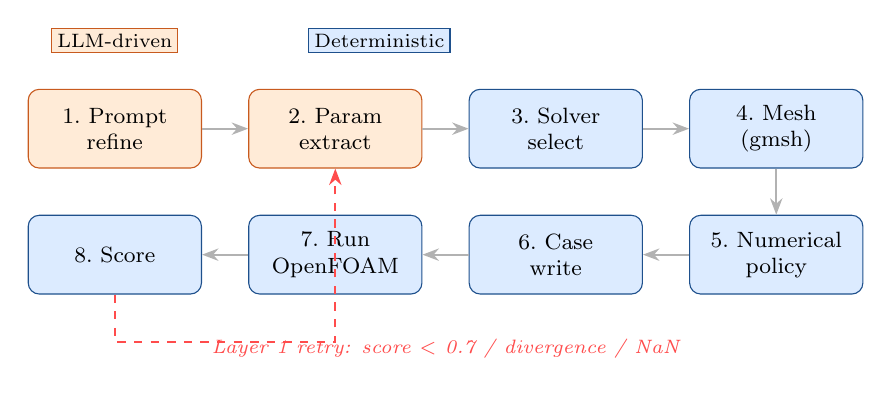
\begin{tikzpicture}[
    every node/.style={font=\footnotesize},
    stage/.style={rectangle, rounded corners, draw=autoBlue, minimum width=22mm,
        minimum height=10mm, align=center, fill=lightBlue, inner sep=2pt},
    llmstage/.style={rectangle, rounded corners, draw=autoOrange, minimum width=22mm,
        minimum height=10mm, align=center, fill=lightOrange, inner sep=2pt},
    arrow/.style={-{Stealth[scale=0.9]}, thick, gray!60},
    x=28mm, y=16mm,
    ]
    % Top row
    \node[llmstage] (n1) at (0,1) {1.~Prompt\\refine};
    \node[llmstage] (n2) at (1,1) {2.~Param\\extract};
    \node[stage]    (n3) at (2,1) {3.~Solver\\select};
    \node[stage]    (n4) at (3,1) {4.~Mesh\\(gmsh)};
    % Bottom row
    \node[stage]    (n5) at (3,0) {5.~Numerical\\policy};
    \node[stage]    (n6) at (2,0) {6.~Case\\write};
    \node[stage]    (n7) at (1,0) {7.~Run\\OpenFOAM};
    \node[stage]    (n8) at (0,0) {8.~Score};
    % Arrows
    \draw[arrow] (n1) -- (n2);
    \draw[arrow] (n2) -- (n3);
    \draw[arrow] (n3) -- (n4);
    \draw[arrow] (n4) -- (n5);
    \draw[arrow] (n5) -- (n6);
    \draw[arrow] (n6) -- (n7);
    \draw[arrow] (n7) -- (n8);
    % Retry
    \draw[arrow, dashed, red!70]
      (n8.south) -- ++(0,-6mm) -| ($(n2.south)+(0,-6mm)$) -- (n2.south);
    \node[font=\scriptsize\itshape, red!70] at (1.5,-0.75)
      {Layer 1 retry: score $<$ 0.7 / divergence / NaN};
    % Legend
    \node[draw=autoOrange, fill=lightOrange, inner sep=2pt, font=\scriptsize] at (0.0,1.7) {LLM-driven};
    \node[draw=autoBlue,   fill=lightBlue,   inner sep=2pt, font=\scriptsize] at (1.2,1.7) {Deterministic};
  \end{tikzpicture}
  \end{center}
  \vspace{-4pt}
  \begin{columns}
    \begin{column}{0.48\textwidth}
      \begin{block}{LLM is invoked only where needed}
        \small Prompt refinement, parameter extraction, RAG context, retry generation
      \end{block}
    \end{column}
    \begin{column}{0.48\textwidth}
      \begin{block}{Deterministic steps ensure correctness}
        \small Solver routing, mesh generation, case writing, execution, scoring
      \end{block}
    \end{column}
  \end{columns}
\end{frame}

\begin{frame}{Key Design Choices}
  \begin{columns}
    \begin{column}{0.48\textwidth}
      \begin{block}{Constrained Parameter Extraction}
        \begin{itemize}
          \item \textbf{vLLM} for high-throughput inference
          \item \textbf{xgrammar} JSON schema enforces \texttt{CFDParams} structure
          \item Output: geometry class, $Re$, fluid properties, solver settings, turbulence model
          \item Post-generation regex validates $Re = UL/\nu$ consistency
        \end{itemize}
      \end{block}
    \end{column}
    \begin{column}{0.48\textwidth}
      \begin{block}{Deterministic Solver Routing}
        \begin{itemize}
          \item Decouples solver choice from LLM
          \item Uses physics flags: transient, compressible, thermal, multiphase
          \item Routes to one of \textbf{7 approved solvers}
          \item Prevents LLM bias (e.g.\ choosing \texttt{simpleFoam} for transient vortex shedding)
        \end{itemize}
      \end{block}
    \end{column}
  \end{columns}
  \vspace{6pt}
  \begin{alertblock}{Multi-Objective Reward $r \in [0,1]$}
    \centering\small
    Convergence (+0.40) $|$ Residual $<10^{-4}$ (+0.20) $|$ Mass conservation (+0.05) $|$ Correct solver (+0.10) $|$ Valid BCs (+0.05)\\
    Penalties: mesh quality, slow runtime, stagnation $(-0.25$ total)
  \end{alertblock}
\end{frame}

% =============================================================================
\section{Dataset Curation}
% =============================================================================

\begin{frame}{Training Data: Static + Dynamic}
  \begin{columns}
    \begin{column}{0.48\textwidth}
      \begin{block}{Foundational Knowledge Corpus}
        \begin{itemize}
          \item \textbf{402 rows} of expert OpenFOAM interaction trajectories
          \item 252 unique prompts covering all solver types and geometry parameterizations
          \item Accepted trajectories: score $r \geq 0.5$
          \item Format: natural language $\to$ summary $\to$ full C++ dictionary blocks
        \end{itemize}
      \end{block}
    \end{column}
    \begin{column}{0.48\textwidth}
      \begin{block}{Dynamic Trajectory Capture}
        \begin{itemize}
          \item Live production runs feed the dataset continuously
          \item High-success runs ($r \geq 0.65$): added to training pool
          \item Currently \textbf{210 de-duplicated topologies}
          \item Failed runs logged with failure type for DPO preference mining
        \end{itemize}
      \end{block}
    \end{column}
  \end{columns}
  \vspace{8pt}
  \begin{exampleblock}{Out-of-Distribution (OOD) Benchmark — 110 Prompts}
    \centering\small
    \begin{tabular}{lrr}
      \toprule
      \textbf{Solver Family} & \textbf{Count} & \textbf{Share} \\
      \midrule
      \texttt{simpleFoam} (steady incompressible) & 74 & 67\% \\
      \texttt{rhoSimpleFoam} (steady compressible) & 9 & 8\% \\
      \texttt{interFoam} (multiphase VOF) & 7 & 6\% \\
      Others (\texttt{buoyantSimpleFoam}, \texttt{pimpleFoam}, ...) & 20 & 18\% \\
      \bottomrule
    \end{tabular}
  \end{exampleblock}
\end{frame}

% =============================================================================
\section{Self-Evolution Pipeline}
% =============================================================================

\begin{frame}{The Seven-Layer Evolution Loop}
  \begin{center}
  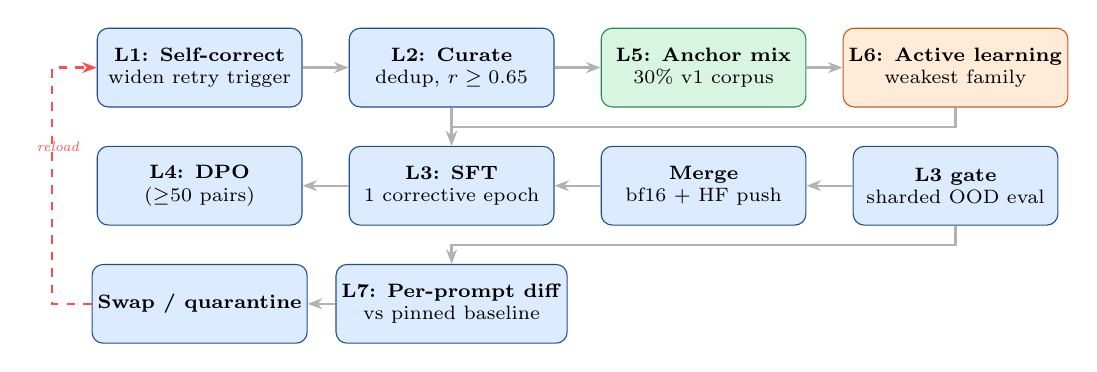
\begin{tikzpicture}[
    every node/.style={font=\scriptsize},
    layer/.style={rectangle, rounded corners, draw=autoBlue, minimum width=26mm,
        minimum height=10mm, align=center, fill=lightBlue, inner sep=2pt},
    anchorbox/.style={rectangle, rounded corners, draw=autoGreen, minimum width=26mm,
        minimum height=10mm, align=center, fill=lightGreen, inner sep=2pt},
    activebox/.style={rectangle, rounded corners, draw=autoOrange, minimum width=26mm,
        minimum height=10mm, align=center, fill=lightOrange, inner sep=2pt},
    arrow/.style={-{Stealth[scale=0.8]}, thick, gray!60},
    x=32mm, y=15mm,
    ]
    % Row 0
    \node[layer]     (n1) at (0,2)  {\textbf{L1: Self-correct}\\widen retry trigger};
    \node[layer]     (n2) at (1,2)  {\textbf{L2: Curate}\\dedup, $r\geq0.65$};
    \node[anchorbox] (n5) at (2,2)  {\textbf{L5: Anchor mix}\\30\% v1 corpus};
    \node[activebox] (n6) at (3,2)  {\textbf{L6: Active learning}\\weakest family};
    % Row 1
    \node[layer]     (l4) at (0,1)  {\textbf{L4: DPO}\\($\geq$50 pairs)};
    \node[layer]     (l3) at (1,1)  {\textbf{L3: SFT}\\1 corrective epoch};
    \node[layer]     (mg) at (2,1)  {\textbf{Merge}\\bf16 + HF push};
    \node[layer]     (gt) at (3,1)  {\textbf{L3 gate}\\sharded OOD eval};
    % Row 2
    \node[layer]     (sw) at (0,0)  {\textbf{Swap / quarantine}};
    \node[layer]     (l7) at (1,0)  {\textbf{L7: Per-prompt diff}\\vs pinned baseline};
    % Arrows
    \draw[arrow] (n1) -- (n2);
    \draw[arrow] (n2) -- (n5);
    \draw[arrow] (n5) -- (n6);
    \draw[arrow] (n6.south) -- ++(0,-2.5mm) -| (l3.north);
    \draw[arrow] (n2.south) -- (l3.north);
    \draw[arrow] (gt) -- (mg);
    \draw[arrow] (mg) -- (l3);
    \draw[arrow] (l3) -- (l4);
    \draw[arrow] (gt.south) -- ++(0,-2.5mm) -| (l7.north);
    \draw[arrow] (l7) -- (sw);
    \draw[arrow, dashed, red!70] (sw.west) -- ++(-5mm,0) |- ($(n1.west)+(-5mm,0)$) -- (n1.west);
    \node[font=\tiny\itshape, red!70, anchor=east] at ($(n1.west)+(-1mm,-10mm)$) {reload};
  \end{tikzpicture}
  \end{center}
  \vspace{-4pt}
  \begin{columns}
    \begin{column}{0.32\textwidth}
      \begin{block}{\footnotesize\color{autoGreen} L5: Anchor Mixing}
        \scriptsize 30\% foundational corpus injected into every retraining batch — prevents catastrophic forgetting
      \end{block}
    \end{column}
    \begin{column}{0.32\textwidth}
      \begin{block}{\footnotesize\color{autoOrange} L6: Active Learning}
        \scriptsize Targets the weakest solver family; auto-generates new seeds to strengthen it
      \end{block}
    \end{column}
    \begin{column}{0.32\textwidth}
      \begin{block}{\footnotesize L7: Regression Firewall}
        \scriptsize Word-by-word diff against pinned baseline before any weight promotion
      \end{block}
    \end{column}
  \end{columns}
\end{frame}

\begin{frame}{Anti-Collapse Mechanisms}
  \begin{block}{The Self-Distillation Collapse Risk}
    Training on self-generated data can rapidly degrade model quality — AutoFOAM deploys \textbf{three complementary defences}.
  \end{block}
  \vspace{6pt}
  \begin{columns}
    \begin{column}{0.32\textwidth}
      \begin{exampleblock}{RAG-Augmented Retry}
        \small
        Chroma vector DB of verified OpenFOAM tutorial configs.\\[4pt]
        Injects relevant dictionary snippets into the retry prompt.
      \end{exampleblock}
    \end{column}
    \begin{column}{0.32\textwidth}
      \begin{exampleblock}{Surgical Dictionary Patching}
        \small
        On localised \texttt{FOAM FATAL} errors, patches only the offending dictionary.\\[4pt]
        Skips costly \texttt{gmsh} remeshing — fast feedback loop.
      \end{exampleblock}
    \end{column}
    \begin{column}{0.32\textwidth}
      \begin{exampleblock}{Prompt Diversity Paraphrasing}
        \small
        Varies semantic structure of training prompts to prevent the model from overfitting to one phrasing pattern.
      \end{exampleblock}
    \end{column}
  \end{columns}
  \vspace{8pt}
  \begin{alertblock}{Layer 4: Direct Preference Optimization (DPO)}
    \centering\small
    Failure trajectory (rejected) $\longleftrightarrow$ Layer-1-corrected success (chosen) \\
    DPO explicitly penalises the syntactic formulations that caused divergence.
  \end{alertblock}
\end{frame}

% =============================================================================
\section{Results}
% =============================================================================

\begin{frame}{Autonomous Case Generation}
  \begin{columns}
    \begin{column}{0.50\textwidth}
      \begin{block}{Coverage}
        \begin{itemize}
          \item \textbf{7 solver families}: \texttt{simpleFoam}, \texttt{pimpleFoam}, \texttt{rhoSimpleFoam}, \texttt{rhoPimpleFoam}, \texttt{buoyantSimpleFoam}, \texttt{interFoam}, \texttt{icoFoam}
          \item \textbf{13 parameterised gmsh geometries}: driven cavity, backward step, NACA airfoil, cylinder, periodic hill, S-bend, Ahmed body, …
          \item Input: \textit{one natural-language sentence}
          \item Output: correct \texttt{polyMesh} boundaries + convergent solution
        \end{itemize}
      \end{block}
    \end{column}
    \begin{column}{0.47\textwidth}
      \begin{exampleblock}{OOD Headline Metrics}
        \centering
        \begin{tabular}{lr}
          \toprule
          \textbf{Metric} & \textbf{Value} \\
          \midrule
          FOAM FATAL-free & \textbf{110/110} \\
          Execution success & \textbf{100\%} \\
          Solver routing accuracy & \textbf{96.4\%} \\
          Mean reward $r$ & \textbf{0.64} \\
          Geometry templates & \textbf{13/13} \\
          Solver families & \textbf{7/7} \\
          \bottomrule
        \end{tabular}
      \end{exampleblock}
    \end{column}
  \end{columns}
  \vspace{4pt}
  \begin{alertblock}{Misrouted Cases}
    \small Only 4/110 solver mismatches — all in \textbf{ambiguous low-Re regimes}
    (e.g.\ transient cylinder at $Re=250$: \texttt{icoFoam} selected instead of \texttt{pimpleFoam} — physically justified).
  \end{alertblock}
\end{frame}

\begin{frame}{Representative OOD Prompts (within geometry support and solver type)}
  \begin{block}{AutoFOAM correctly maps natural language $\to$ physics $\to$ solver}
  \end{block}
  \vspace{4pt}
  \small
  \begin{tabularx}{\textwidth}{lXll}
    \toprule
    \textbf{Tag} & \textbf{Prompt} & \textbf{Predicted Solver} & \textbf{Match} \\
    \midrule
    \texttt{cav\_re150} & \emph{Cavity flow Re=150 in water, 0.4~m square} & \texttt{simpleFoam} & \checkmark \\
    \texttt{pipe\_lam} & \emph{Laminar pipe flow Re=500, diameter 0.02~m, water} & \texttt{simpleFoam} & \checkmark \\
    \texttt{naca\_re1m} & \emph{NACA0012 at Re=$10^6$, 5$^\circ$ angle of attack} & \texttt{simpleFoam} & \checkmark \\
    \texttt{dam\_tall} & \emph{Tall dam break, 2~m wide, 5~m water column collapse} & \texttt{interFoam} & \checkmark \\
    \texttt{cdnoz\_ma04} & \emph{Convergent-divergent nozzle with Mach 0.4 throat, air} & \texttt{rhoSimpleFoam} & \checkmark \\
    \texttt{cyl\_re250} & \emph{Transient cylinder Re=250 in water, D=0.1~m} & \texttt{icoFoam} & $\times$ \\
    \bottomrule
  \end{tabularx}
  \vspace{6pt}
  \begin{block}{Evaluation Infrastructure}
    8-way sharded cluster of \textbf{NVIDIA H100} GPUs — 110 OOD prompts in isolation from training data
  \end{block}
\end{frame}

\begin{frame}{Live Demo}
  \begin{columns}[c]
    \begin{column}{0.58\textwidth}
      \href{https://www.youtube.com/watch?v=Kx17bfFlMSc}{%
        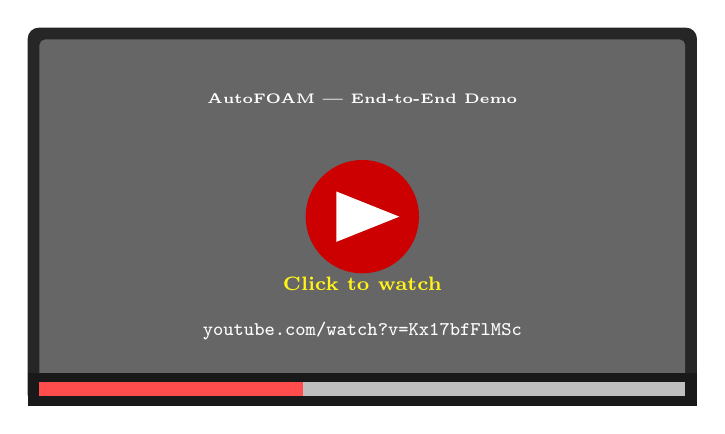
\begin{tikzpicture}
          % Video frame background
          \fill[black!85, rounded corners=4pt] (0,0) rectangle (8.5,4.8);
          % Inner screen area
          \fill[black!60, rounded corners=2pt] (0.15,0.15) rectangle (8.35,4.65);
          % Red YouTube play button circle
          \fill[red!80!black] (4.25,2.4) circle (0.72);
          % White play triangle
          \fill[white] (3.92,2.08) -- (3.92,2.72) -- (4.72,2.40) -- cycle;
          % Bottom bar
          \fill[black!90] (0,0) rectangle (8.5,0.42);
          % Progress bar (partially filled)
          \fill[red!70] (0.15,0.12) rectangle (3.5,0.30);
          \fill[gray!50] (3.5,0.12) rectangle (8.35,0.30);
          % URL text on screen
          \node[white, font=\scriptsize\ttfamily] at (4.25,0.95)
            {youtube.com/watch?v=Kx17bfFlMSc};
          \node[white!80, font=\tiny] at (4.25,3.9) {\textbf{AutoFOAM — End-to-End Demo}};
          % Click hint
          \node[yellow!90, font=\scriptsize\bfseries] at (4.25,1.55)
            {Click to watch};
        \end{tikzpicture}%
      }
    \end{column}
    \begin{column}{0.38\textwidth}
      \begin{block}{What the Demo Shows}
        \begin{itemize}
          \item Natural-language prompt input
          \item Automated parameter extraction
          \item \texttt{gmsh} mesh generation
          \item OpenFOAM case file synthesis
          \item Live solver run + convergence
          \item Velocity contour output
        \end{itemize}
      \end{block}
      \vspace{6pt}
      \begin{exampleblock}{Watch Online}
        \centering\small
        \href{https://www.youtube.com/watch?v=Kx17bfFlMSc}%
          {\texttt{youtu.be/Kx17bfFlMSc}}
      \end{exampleblock}
    \end{column}
  \end{columns}
\end{frame}

\begin{frame}{Automatically Generated Meshes}
  \begin{columns}[c]
    \begin{column}{0.48\textwidth}
      \begin{figure}
        \includegraphics[width=\linewidth,height=2.5cm,keepaspectratio]{airfoil_mesh_zoom_wide.png}
        \caption{\small NACA-4-digit airfoil}
      \end{figure}
      \begin{figure}
        \includegraphics[width=\linewidth,height=2.5cm,keepaspectratio]{clean_periodic_hill_mesh.png}
        \caption{\small Periodic hill (Mellen polynomial)}
      \end{figure}
    \end{column}
    \begin{column}{0.48\textwidth}
      \begin{figure}
        \includegraphics[width=\linewidth,height=2.5cm,keepaspectratio]{cylinder_mesh_zoom.png}
        \caption{\small Cylinder in cross-flow}
      \end{figure}
      \begin{figure}
        \includegraphics[width=\linewidth,height=2.5cm,keepaspectratio]{clean_sbend_mesh.png}
        \caption{\small S-bend duct}
      \end{figure}
    \end{column}
  \end{columns}
  \vspace{-4pt}
  \begin{block}{}
    \centering\small All meshes generated fully autonomously from a single natural-language prompt via \texttt{gmsh}
  \end{block}
\end{frame}

\begin{frame}{Velocity Contours — Autonomous Flow Solutions}
  \begin{columns}[c]
    \begin{column}{0.48\textwidth}
      \begin{figure}
        \includegraphics[width=\linewidth,height=2.5cm,keepaspectratio]{airfoil_zoom_mid.png}
        \caption{\small NACA-4-digit airfoil — velocity magnitude}
      \end{figure}
      \begin{figure}
        \includegraphics[width=\linewidth,height=2.5cm,keepaspectratio]{clean_periodic_hill_velocity.png}
        \caption{\small Periodic hill — velocity magnitude}
      \end{figure}
    \end{column}
    \begin{column}{0.48\textwidth}
      \begin{figure}
        \includegraphics[width=\linewidth,height=2.5cm,keepaspectratio]{cylinder_zoom_mid.png}
        \caption{\small Cylinder in cross-flow — velocity magnitude}
      \end{figure}
      \begin{figure}
        \includegraphics[width=\linewidth,height=2.5cm,keepaspectratio]{clean_sbend_velocity.png}
        \caption{\small S-bend — velocity magnitude}
      \end{figure}
    \end{column}
  \end{columns}
  \vspace{-4pt}
  \begin{block}{}
    \centering\small No manual intervention — correct \texttt{polyMesh} boundaries and convergent solutions generated end-to-end
  \end{block}
\end{frame}

% =============================================================================
\section{Limitations \& Future Work}
% =============================================================================

\begin{frame}{Scope, Limitations, and Next Steps}
  \begin{columns}
    \begin{column}{0.48\textwidth}
      \begin{alertblock}{Current Limitations}
        \begin{itemize}
          \item \textbf{Geometry}: restricted to 13 parameterised \texttt{gmsh} models — no raw CAD (STEP/IGES) support
          \item \textbf{Physics}: RANS-only turbulence; no LES/DNS
          \item \textbf{Reward}: biased toward mathematical convergence — a numerically sound solution can still be \textit{physically wrong} (e.g.\ incorrect drag coefficient)
          \item No cross-reference against benchmark databases (e.g.\ Ghia cavity data)
        \end{itemize}
      \end{alertblock}
    \end{column}
    \begin{column}{0.48\textwidth}
      \begin{exampleblock}{Future Work}
        \begin{itemize}
          \item \textbf{Physics Validator}: external module comparing agent output against known benchmark data — closes the physics-validation gap
          \item CAD-to-mesh pipeline for complex industrial geometries
          \item LES/DNS numerical policy
          \item Broader solver coverage (e.g.\ \texttt{reactingFoam}, \texttt{chtMultiRegionFoam})
          \item Tighter DPO negative feedback once physics validator is live
        \end{itemize}
      \end{exampleblock}
    \end{column}
  \end{columns}
\end{frame}

% =============================================================================
\section{Conclusion}
% =============================================================================

\begin{frame}{Conclusion}
  \begin{block}{What We Built}
    \textbf{AutoFOAM} — a self-refining LLM agent that closes the semantic gap between natural-language intent and correct OpenFOAM simulation execution.
  \end{block}
  \vspace{6pt}
  \begin{columns}
    \begin{column}{0.48\textwidth}
      \textbf{Key Contributions}
      \begin{itemize}
        \item \textbf{Autonomous CFD Agent}: Qwen2.5-Coder-14B fine-tuned on 252 CFD-specific prompts; syntactically sound and physically consistent output
        \item \textbf{Seven-Layer Evolution Loop}: SFT + DPO + anchor mixing + active learning + regression gate — monotonic performance improvement
        \item \textbf{Anti-Collapse Strategies}: RAG retry, surgical patching, prompt paraphrasing
      \end{itemize}
    \end{column}
    \begin{column}{0.48\textwidth}
      \begin{exampleblock}{Key Results}
        \centering\large
        \textbf{100\%} execution success\\[4pt]
        \textbf{96.4\%} solver routing accuracy\\[4pt]
        \textbf{13/13} geometry templates\\[4pt]
        \textbf{7/7} solver families
      \end{exampleblock}
      \vspace{4pt}
      \begin{block}{Open Source}
        \scriptsize
        Code: \href{https://github.com/AGN000/AutoFOAM}{\texttt{github.com/AGN000/AutoFOAM}}\\
        Data: \href{https://github.com/AGN000/FoamAgentCases}{\texttt{github.com/AGN000/FoamAgentCases}}\\
        Weights: \href{https://huggingface.co/arungovindneelan/foam-cfd-unified-14b}{\texttt{hf.co/arungovindneelan/foam-cfd-unified-14b}}
      \end{block}
    \end{column}
  \end{columns}
  \vspace{4pt}
  \centering\small\textit{Supported by the \textbf{NVIDIA Inception} programme}
\end{frame}

% ── Thank you ────────────────────────────────────────────────────────────────
\begin{frame}{}
  \centering
  \vspace{20pt}
  {\Huge\color{autoBlue}\textbf{Thank You}}\\[12pt]
  {\large Questions \& Discussion}\\[20pt]
  \begin{columns}
    \begin{column}{0.45\textwidth}
      \begin{block}{Contact}
        Arun Govind Neelan\\
        \texttt{arungovindneelan@gmail.com}\\[4pt]
        A Seshaditya\\
        \texttt{adi@onnes.in}
      \end{block}
    \end{column}
    \begin{column}{0.45\textwidth}
      \begin{block}{Resources}
        \scriptsize
        \href{https://github.com/AGN000/AutoFOAM}{\texttt{github.com/AGN000/AutoFOAM}}\\
        \href{https://huggingface.co/arungovindneelan/foam-cfd-unified-14b}{\texttt{huggingface.co/arungovindneelan/\ldots}}
      \end{block}
    \end{column}
  \end{columns}
\end{frame}

\end{document}
